
\section{Pipes: A real world example}
\label{sec:pipes}
\todo{Abschnitt neu formulieren oder wegglassen}
Pipes is a streaming library for Haskell. It was build with the following requirements \cite{gonzales13}.
\begin{description}
\item[Effects] Streams has to be effectful
\item[Streaming] Processing in constant memory
\item[Composability] Modules have to be composable
\end{description}

Pipes uses the type class \verb|Category| too keep the API simple and easy to use.

This article will descipe a part of the library with an example.

First we need a input stream, that emits values. Input streams are have the type 
\verb|Producer a m ()|.
Listing \ref{lst:simpleproducer} show a simple Producer. It emits the integers 1,2 and 3. It is also possible to create producers for effectful streams. We use the simple producer from Listing \ref{lst:simpleproducer} for simplicity reasons.

\begin{program}
\begin{verbatim}
produceints123 :: Producer Int IO ()
produceints123 = each [1,2,3]
\end{verbatim}
\caption{Simple Producer}
\label{lst:simpleproducer}
\end{program}

Pipes provide the function \verb|for| to consume a producer. 
\verb|for| \verb|producer| \verb|body| loops over the \verb|producer| and applies a the transformation defined in \verb|body| to every element yielded by the producer. If the body is of type \verb|Effect| it return an \verb|Effect|. If body is of type \verb|Producer| a \verb|Producer| is returned. The type declaration of \verb|for| 
\begin{program}
\begin{verbatim}
for::Monad m=>
Producer b m r
-> (b -> Producer c m ())
-> Producer c m r
\end{verbatim}
\caption{type of for}
\end{program}

A value for the body, could be function, that takes \verb|Int| and returns producer \verb|Producer a IO ()|. Hence the type declarion is \verb|Int -> Producer a IO ()|. We implement a body, that prints the integers to the standard input (strictly speaking this value is an effect of type \verb|Effect Int ()|. But \verb|Effect Int ()| is of type \verb|Producer Int IO () |).

\begin{program}
\begin{verbatim}
print2stdout:: Int -> Effect IO ()
print2stdout x = (lift . putStrLn . show ) x
\end{verbatim}
\caption{Definition of an effect, that prints to stdout}
\label{lst:stdouteffect}
\end{program}

With the producer and the body we can define a \verb|Effect IO ()|
\begin{verbatim}
effect :: Effect IO ()
effect = for produceints123 print2stdout
\end{verbatim}

Because the \verb|body| and of \verb|for| can be of type \verb|a -> Producer|, and the type of the return value is \verb|Producer|, it's possible to interleave several Producers.

If we want to duplicate all element we write another body
\begin{verbatim}
duplicate :: Int -> Producer Int IO ()
duplicate x = yield x >> yield x 
\end{verbatim}

We use \verb|for| to create a another producer. \verb|composed_producer| is a composition of \verb|produceints123| and \verb|duplicate|.
\begin{verbatim}
composed_producer :: Producer Int IO ()
composed_producer = for produceints123 duplicate
\end{verbatim}

To compose \verb|composed_producer| with our \verb|print2stdout| effect, we apply the \verb|for| function

\begin{verbatim}
effect2 :: Effect IO ()
effect2 = for composed_producer print2stdout
\end{verbatim}

In order to compose producers, the pipe library provides the \verb|~>| function. \verb|~>| is defined as follows:
\begin{verbatim}
(f ~> g) x = for (f x) g
\end{verbatim}

Hence we can write compose a body for \verb|for| like this:
\begin{verbatim}
composed_with_yield :: Int -> Effect IO ()
composed_with_yield = duplicate ~> print2stdout
\end{verbatim}

Gabriel Gonzales proved that the \verb|~>| operator is associativ. It has the associativity property.

\begin{verbatim}
 -- Associativity
 (f ~> g) ~> h = f ~> (g ~> h)
\end{verbatim}

Because the \verb|~>| operator is associativ, it doesnt matter in witch order the body is composed. The expected behavior is defined in term of cateory laws. It's possible to prove that the specified laws hold.

\section{Appendix}
\label{sec:appendix}

\subsection{Applicative Functor}
\label{sec:applicatives}

Applicative functors are an abstract characterization of an applicative style of effectful programming \cite{mcbride} \cite{control.applicative}

The \verb|Applicative| type class encapsulates the following idea. What if you have a function wrapped in a \verb|Functor| (e.g. \verb|Maybe (Int -> Int -> Int)|) and you want to apply the function to another functor (e.g. \verb|Maybe Int|). For example we want to map \verb|Just (3 *)|, a function encapsulated inside a functor, over \verb|Just 23|, another functor with an encapsulated \verb|Int|? \verb|fmap| doesn't work here, because it expects a normal function \verb|a -> b| as first parameter. That's where the \verb|Applicative| type class come in. 
The \verb|Applicative| type class is defined as follows \cite{control.applicative}.
\begin{verbatim}
class (Functor f) => Applicative f where
    pure :: a -> f a
    (<*>) :: f (a -> b) -> f a -> f b
\end{verbatim}

The type class declaration demands the type \verb|f| to be a functor. Every type that is part of \verb|Applicative| is part of \verb|Functor|. Hence we can use \verb|fmap| with \verb|Applicative| instances.
Applicatives are enhanced functors. In addition to to \verb|fmap| we can use the \verb|<*>| operator to chain several applicative values together.

The \verb|pure| function puts a value of type \verb|a| in a default context. If applied with a function \verb|a -> b| pure return a functor with a function inside, hence the first argument to \verb|<*>|.

It possible to chain applicative together as follows:
\begin{verbatim}
ghci> pure (*) <*> Just 3 <*> Just 23
Just 69
\end{verbatim}

The following type are instances of the type class \verb|Applicative| \todo{instances beschreiben}

\begin{itemize}
\item Maybe
\item Lists
\item IO
\end{itemize}

There are several laws that \verb|Applicative| instances should satisfy \cite{mcbride} \cite{control.applicative}. This article will use only the following :

\begin{enumerate}
\item \verb|pure id <*> v = v|
\item \verb|fmap g x = pure g <*> x|
\item \verb|pure f <*> pure x = pure (f x)|
\end{enumerate}

\todo{Handskizzen durch grafik ersetzen}The second law says that applying \verb|fmap| over a normal function \verb|g| over a functor \verb|x| is the same as putting \verb|g| in a default context and mapping the resulting function over \verb|x|. Figure \ref{fig:functor_applicative} illustrates the relation between \verb|Functor| and \verb|Applicative|.

The third law says that it doesn't matter if we put the values \verb|f| and \verb|x| in a default context first and then apply \verb|<*>| or if we call \verb|f| on \verb|x| first and then put them in a default context. We will use this property to prove another property in section \ref{sec:exampleproof}

\begin{figure}
  \centering
     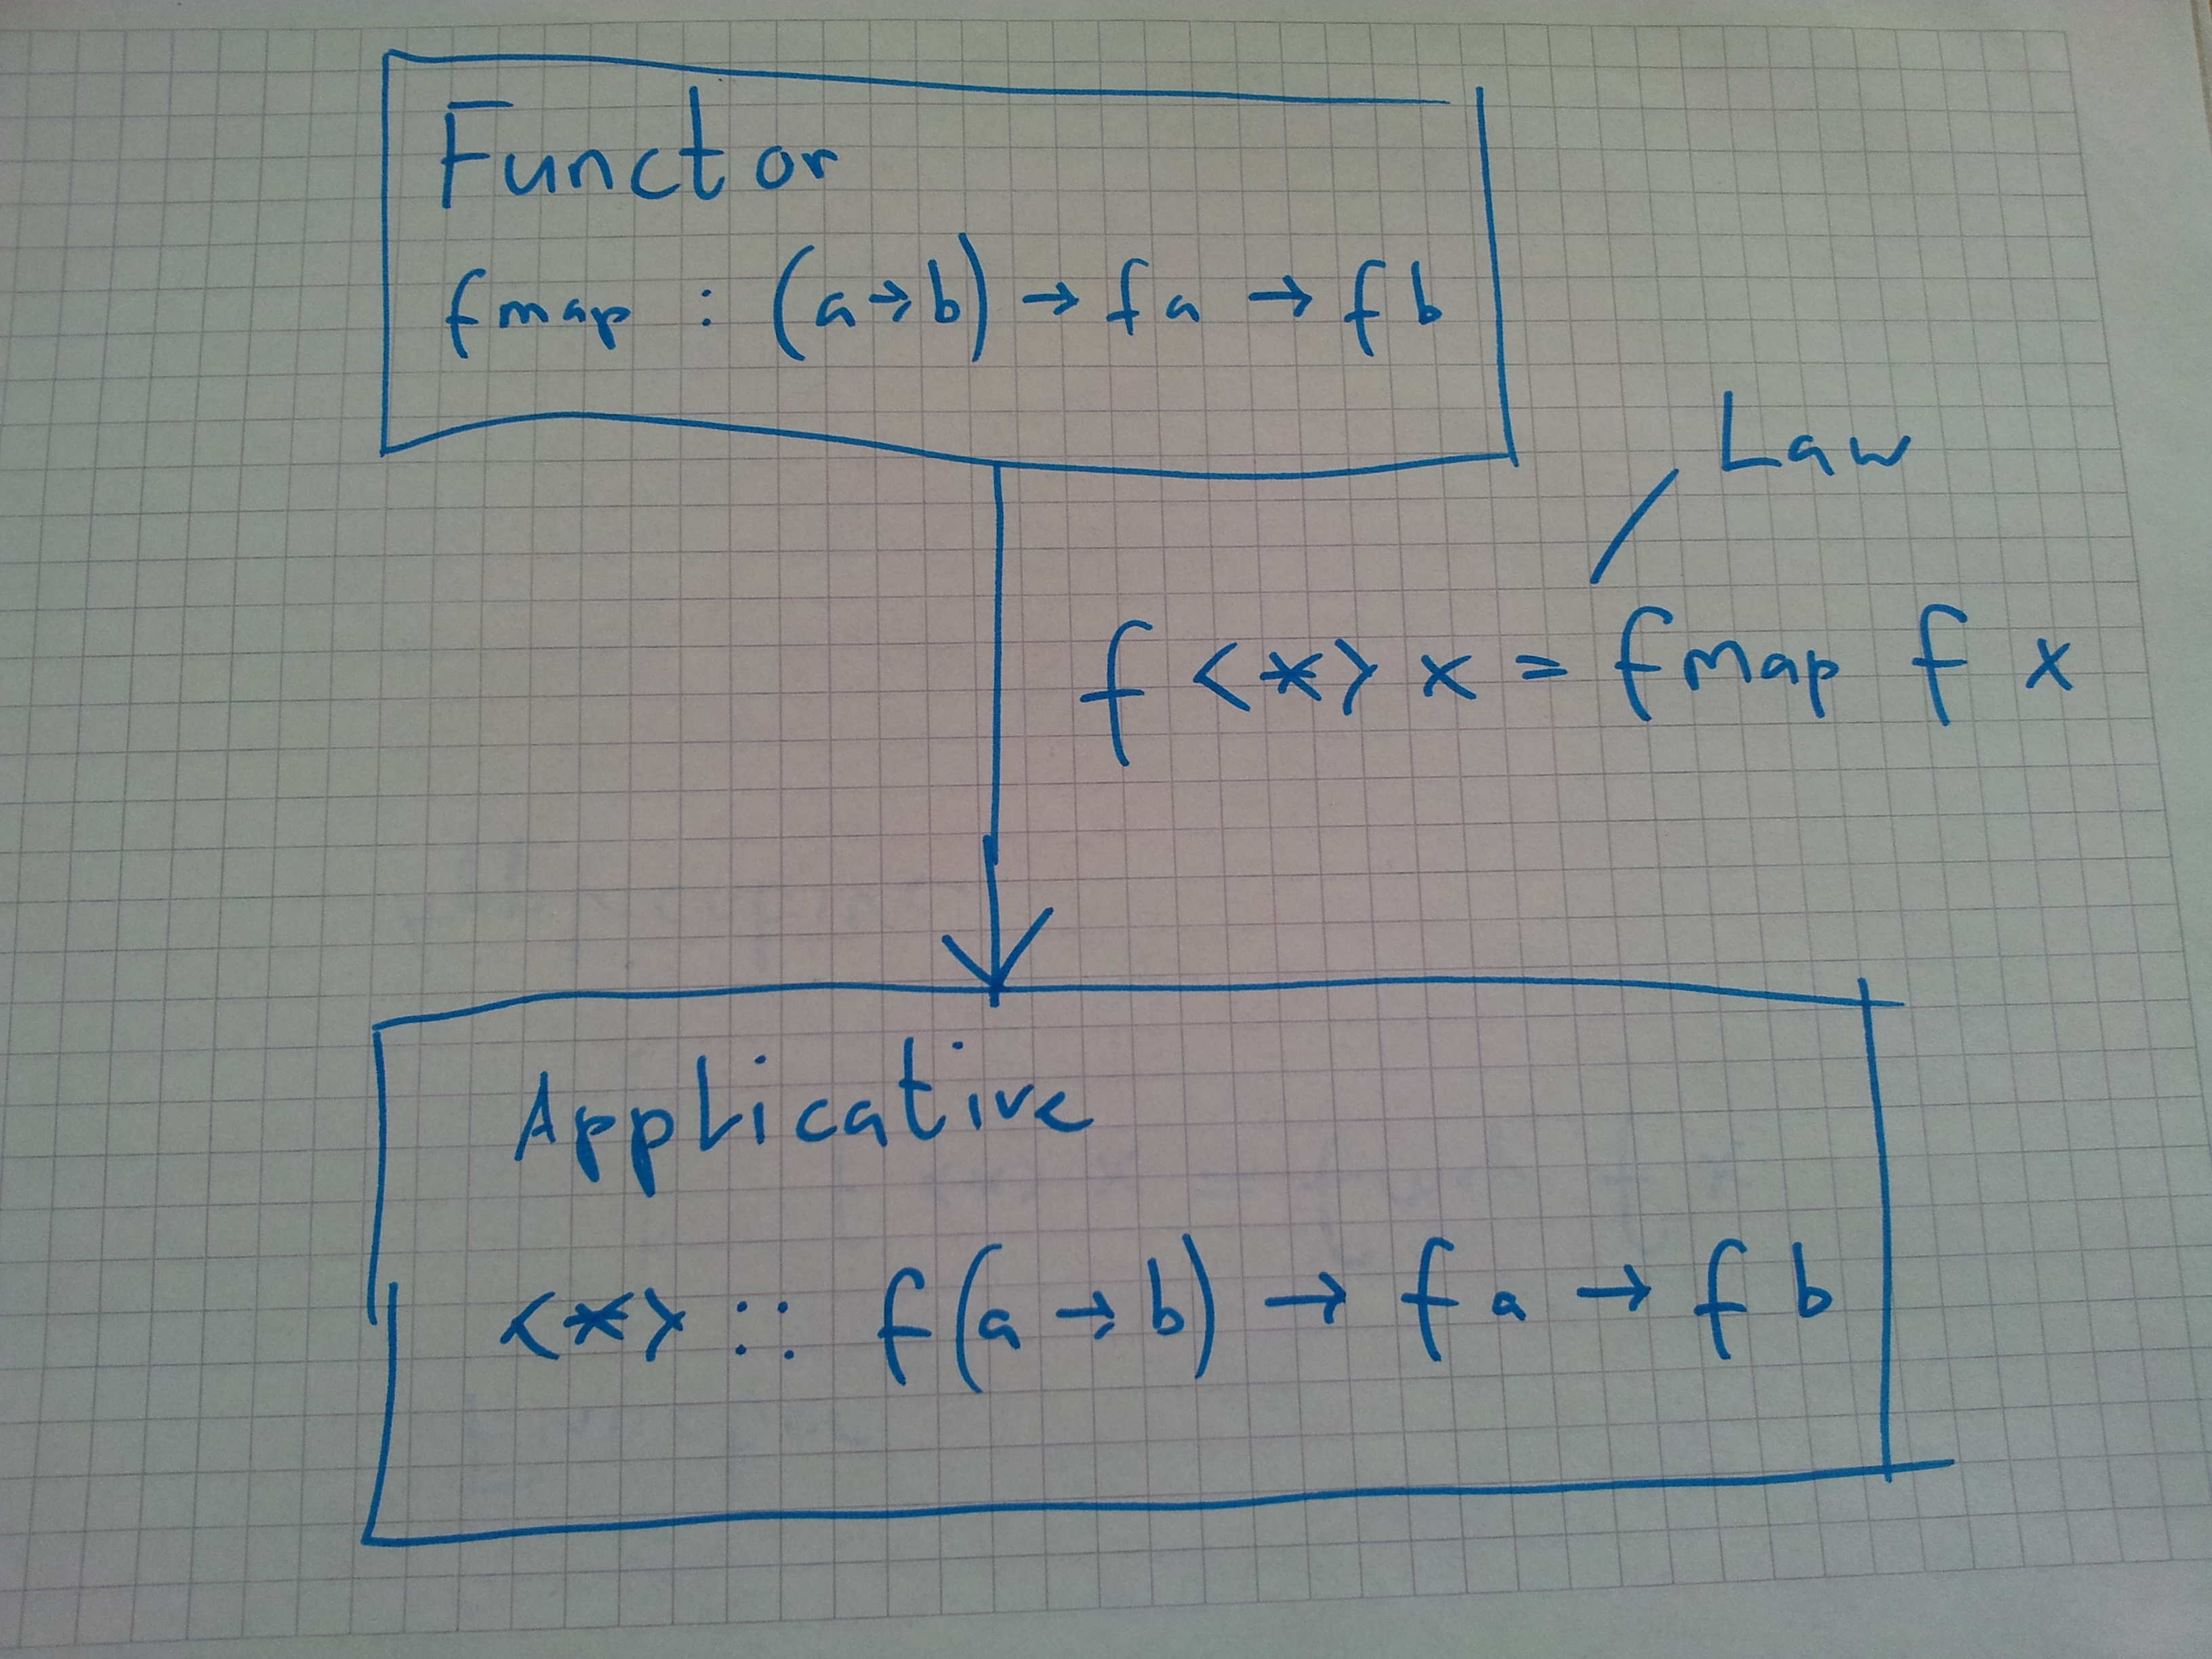
\includegraphics[width=0.9\textwidth]{functor_applicative}
  \caption{Interrelationship of Functor and Applicative }
  \label{fig:functor_applicative}
\end{figure}

\subsection{Function composition}

\label{sec:functioncomposition}

Function composition in mathematics is defined as

\begin{equation}
  \label{eq:functioncomposition}
  (f \circ g)(x) = f(g(x))
\end{equation}

Haskell functions can be compose with the \verb|.| function.

\begin{figure}
  \centering
\begin{verbatim}
(.) :: (b -> c) -> (a -> b) -> a -> c
f . g = \x -> f (g x)
\end{verbatim}
  \caption{. function}
  \label{fig:compositionfunction}
\end{figure}

Function composition allows us to create a function by composing it with many small functions. 

Functions in Haskell form a category in category theory. They satisfy the category laws.


\subsection{Applicative function definition}
 The applicative instance is defined as follows:
\begin{verbatim}
instance Monoid b => Monoid (a -> b) where
    mempty = pure mempty

    mappend = liftA2 mappend
\end{verbatim}

\begin{description}
\item[Associativity law] 
\item[Left/Right Identity law] 
\end{description}

\subsection{garbage}
 There are several methods to verify software.
being able to replace equals by equals.
In this article we will look at technique of equational reasoning to prove type class laws. If we can rely on known properties of your program, we minimize unexpected behavior.


 In addition, they exhibit certain properties. These properties are called laws. 


For example the type class \verb|Functor| makes sure that we can apply the function \verb|fmap| with a type that is part of the \verb|Functor| type class. The type class dictates the behavior. All functors are expected to exhibit certain kinds of properties. These properties guarantee that the function \verb|fmap| only applies a function to all values inside the functor and doesn't change the structure or the context. The expression
\begin{verbatim}
dontchangecontext = do line <- fmap reverse getLine
                       putStrLn $ " "
\end{verbatim}
applies \verb|reverse| to the result of the IO function \verb|getLine| without changing the the input stream. 

Type class instances from the standard library obey the type class laws. If we write new instances, it's our responsibility to check if the type class laws hold.
It's in the responsibility of the programmer to check if the program behaves correctly. For most programmers it's hard to write a correct program at the first attempt. This leaves us with the question of how to verify the type class laws. 

Properties are specified in form of equations. The source code must satisfy this equations. 


The monoid laws are specified by the type class monoid.


\subsection{Functor}
\label{sec:functor}

Functor is a type class for types, which can be mapped over. Another way to describe functors is, that they represent some sort of computational context \cite{yorgey}. The general concept of a functor is more abstract and harder to grasp than the concepts of type classes described above \footnote{this is personal impression}.
The most accurate way to describe the type class \verb|Functor| is to give it's declaration \cite{data.functor}:

\begin{verbatim}
class Functor f where
    fmap :: (a -> b) -> f a -> f b
\end{verbatim}

The \verb|f| in the declaration is a type class constructor. Only type constructor can implement \verb|Functor| (\verb|Maybe|, \verb|[]|).

\verb|fmap| takes any function \verb|a -> b| and a value of type \verb|f a| (\verb|f| is the container or context, \verb|a| is the type wrapped inside the functor) and returns a value of type \verb|f b|. 
If \verb|f a| is of type \verb|Maybe| \verb|Int| and the function of type \verb|Int -> String|, \verb|fmap| returns \verb|Maybe String|. 

Instances of \verb|Functor| are:

\begin{description}
\item[List] \verb|map| for lists for is the same as \verb|fmap|.
\item[Either] \verb|Either e a| is a container. \verb|fmap| applies a function to \verb|a|.
\end{description}

To make a type an instance of \verb|Functor|, it has to define \verb|fmap|. In addition the instances of are expected to exhibit certain kinds of properties. The declaration of the type class doesn't reveal this properties. There are described in the type class documentation \cite{data.functor} \cite{Marlow_2010}. This properties are called the functor laws.
The Haskell Compiler doesn't detect violations of the expected laws. All Functor instances in the standard library obey these laws \cite{yorgey} \cite{Lipovaca}.

A Functor instance has to satisfy the following laws.

\begin{description}
\item[Law 1] Mapping the identity function over a functor value, will not change the functor value. Formally
\begin{verbatim}
fmap id  ==  id
\end{verbatim}
\item[Law 2] It doesn't matter if we compose two functions and them map them over a functor or if we first map one function over the functor and then map the other function. Formally
\begin{verbatim}
fmap (g . h) = fmap g . fmap h
\end{verbatim}
This is the same as \verb|fmap (g . h) = fmap g (fmap h)|
\end{description}

If we can prove that a type satisfies these laws, we can make assumptions about how the the type will act. We know that \verb|fmap| will not change the structure or the context of the functor.
And we know that \verb|fmap| only maps the function over the functor and nothing else. 

If we know, that a type satisfy the laws, we are able to deduce further properties for our own types. In section \ref{sec:example} give an example of this process.

\begin{figure}
  \centering
\begin{verbatim}
fmap id = id
fmap (g . h) = fmap g . fmap h
\end{verbatim}
  \caption{The Functor laws}
  \label{fig:functorlaws}
\end{figure}

A type classes are often compared to interfaces. It contains the function declarations. A type becomes an instance of a type class when it defines all required functions of the type class. When a type is an instance of a type class, we can make certain assumptions about behavior of the type. In contrary to interfaces, type classes aren't types. A value can have the type of an interface but not of a type class. Another difference to interfaces is that type classes describe functions and the instance types are part of the function signature. The instance type can be the return type. Interfaces define methods of the instance type.

The concept of a type class is explained by example with the function \verb|show| from the \verb|Prelude|-Library (\verb|Prelude| is a module and part of the standard). \verb|show| converts a given value of a type \verb|a| into a character string. The type of \verb|show| is

\begin{verbatim}
show :: Show a => a -> String
\end{verbatim}

The \verb|Show a| before the \verb|=>| is a type class constraint. \verb|a| is a type variable. A type that has one more type variables is called polymorphic \cite{hutton}. The signature means that \verb|show| takes something that implements the type class \verb|Show| and returns a string. \verb|Show| is a type class. It's possible to call \verb|show| with different types (e.g \verb|show 1|, \verb|show "hello"|). The compiler will look up the correct definition for us as long the type of the first parameter is an instance of the type class \verb|Show|.  
Any type that implements \verb|Show| can be converted to a character string. Types in this class are \verb|Bool|, \verb|Char|, \verb|Int|, \verb|Float|, \verb|Double| etc.

The type class \verb|Show| is defined as follows:
\begin{verbatim}
class Show a where
    show :: a -> String
\end{verbatim}
The keyword \verb|class| defines a new type class. \verb|a| is the type variable. It represents the type that implements the type class (e.g. \verb|Int| or \verb|Bool|).

Once we have a type class we are able to create instances of that class. The following listing defines a type \verb|Person|. It has fields for name and email address. \todo{loesung fuer schoene listings mit labels und caption finden und ueberall gleich machen}
\begin{verbatim}
data Person = Person { name :: String
                       email :: String
                     }
\end{verbatim}

To make \verb|Person| an instance of \verb|Show| we provide a function with the following type:
\begin{verbatim}
show :: Person -> String|
\end{verbatim}

\begin{verbatim}
instance Show Person where
    show (Person name _) = name
\end{verbatim}

There many other useful type classes in the standard library.

\begin{description}
\item[Ord] Types with an order relation implement \verb|Ord|.
\item[Eq] For types that can be equated.
\item[Read] Types that can be converted from a string.
\end{description}

It will explain the relation to polymorphism and describe type classes \verb|Functor|, \verb|Applicative| and \verb|Monoid| in more detail as these type classes are important for the example in section \ref{sec:example}.

Type classes allow programmers to write general definitions in a typesafe manner by use constrain the paramaters.

Polymorphic functions can be applied to values with different types. 

If a type can be converted to a string, it can be given the type class \verb|Show|. The type \verb|Person| has to provide an implementation for the function \verb|show|. Applying \verb|show| to \verb|Person| results in a different behavior then applying \verb|show| to an \verb|Int|.

\subsection{Monoid}

Some types, let's say \verb|a|, have a binary function with the type declaration. 
\begin{verbatim}
f :: a -> a -> a
\end{verbatim}

The type \verb|a| has a value that serves as identity for the given function. For example the number 1 is the identity for the multiplication. Multiplication of the identity and any other number $x$ results always in $x$.

Several value of type \verb|a| can always be reduces to a single value. It doesn't matter in which order we apply the function, the result is always the same. This is called associativity.

If type \verb|a| has this behavior, it's a monoid and it can be an instance of the \verb|Monoid| type class.


The \verb|Monoid| type class is define as follows \cite{monoid}:
\begin{verbatim}
class Monoid m where
    mempty :: m
    mappend :: m -> m -> m
    mconcat :: [m] -> m
    mconcat = foldr mappend mempty
\end{verbatim}
\verb|mconcat| takes a list of monoids and reduces them \verb|mappend| to a single value, applying mappend. It has a default implementation.

and \verb|mappend| must be associative. There are three monoid laws \cite{monoid}. This article deals only with the first law:

\begin{enumerate}
\item \verb|mappend mempty x = x|
\item \verb|mappend x mempty = x|
\item \verb|(x `mappend y) `mappend z = x `mappend (y `mappend z)|
\end{enumerate}

The following Haskell types are \verb|Monoid| instances
\begin{description}
\item[List] The empty list \verb|[]| and \verb|++| (concatenation) form a monoid.
\item[Product and Sum] Numbers can be monoid with respect to multiplication or addition. There are two monoid instances for \verb|Num|. One for multiplication an the other for addition.
\item[Maybe] Can also be an instance of \verb|Monoid|. \todo{instance beschreiben}
\end{description}

Some types, let's say \verb|a|, have a binary function with the type declaration. 
\begin{verbatim}
f :: a -> a -> a
\end{verbatim}

The type \verb|a| has a value that serves as identity for the given function. For example the number 1 is the identity for the multiplication. Multiplication of the identity and any other number $x$ results always in $x$.

Several value of type \verb|a| can always be reduces to a single value. It doesn't matter in which order we apply the function, the result is always the same. This is called associativity.

If type \verb|a| has this behavior, it's a monoid and it can be an instance of the \verb|Monoid| type class.


The \verb|Monoid| type class is define as follows \cite{monoid}:
\begin{verbatim}
class Monoid m where
    mempty :: m
    mappend :: m -> m -> m
    mconcat :: [m] -> m
    mconcat = foldr mappend mempty
\end{verbatim}
\verb|mconcat| takes a list of monoids and reduces them \verb|mappend| to a single value, applying mappend. It has a default implementation.

and \verb|mappend| must be associative. There are three monoid laws \cite{monoid}. This article deals only with the first law:

\begin{enumerate}
\item \verb|mappend mempty x = x|
\item \verb|mappend x mempty = x|
\item \verb|(x `mappend y) `mappend z = x `mappend (y `mappend z)|
\end{enumerate}

The following Haskell types are \verb|Monoid| instances
\begin{description}
\item[List] The empty list \verb|[]| and \verb|++| (concatenation) form a monoid.
\item[Product and Sum] Numbers can be monoid with respect to multiplication or addition. There are two monoid instances for \verb|Num|. One for multiplication an the other for addition.
\item[Maybe] Can also be an instance of \verb|Monoid|. \todo{instance beschreiben}
\end{description}

All members of the collection  with the property that certain functions are defined over the type.